\documentclass[11pt]{article}
\usepackage[margin=1in]{geometry}
\usepackage{graphicx,booktabs,caption,hyperref,amsmath}
\usepackage[authoryear,round]{natbib}
\hypersetup{colorlinks=true,linkcolor=black,citecolor=black,urlcolor=blue}
\captionsetup{font=small,labelfont=bf}
\setlength{\parskip}{4pt}
\graphicspath{{../results/}}

\title{\textbf{Political Risk and the Global Equity Mix}\\[4pt]
\large Evidence from Ten Equity Markets, 2008--2026}
\author{Divvy Gupta\\ \small\href{https://github.com/divvygupta}{github.com/divvygupta}}
\date{October 2026}

\begin{document}
\maketitle

\begin{abstract}
\noindent This paper asks how a multi-asset fund should account for political risk across its country equity exposures. I build a monthly Political Risk Index (PRI) for ten markets from the Economic Policy Uncertainty and Geopolitical Risk indices and estimate its effects with panel local projections, a fixed-effects panel VAR, and a market-model event study of 30 political events. The results point to political risk as a volatility risk rather than a return risk. A one-standard-deviation political-risk surprise raises a country's realised volatility by about 2\% relative to other markets in the same month ($p = 0.003$), while its effect on excess returns is small ($-0.26$ pp) and reverses within a quarter. Event type matters. Unscheduled governance shocks, such as finance-minister dismissals and leadership scandals, cost $-4.8\%$ over three days on average ($p = 0.02$), while scheduled elections have no significant effect. A rule that underweights markets with rising political risk adds little (information ratio 0.16). Four forward-looking scenarios, each calibrated to a historical episode, show that tariff escalation or a European security crisis would raise a Canadian-dollar portfolio's one-month value at risk by about 11--12\%. They also show that the U.S. dollar's role as a safe haven depends on the crisis, and that news-based indices miss domestic governance shocks. Across 50 national elections, what moves markets is the polling error, not the election: results that went against the final polls moved stocks by 3.6 times a normal day, against 1.1 times when the polls were right ($p = 0.01$). Resignations of heads of government rarely matter, exogenous shocks leave volatility elevated for longer than scheduled events, and thematic risks build up over months rather than in a single day. Political risk is best treated as an input to the risk budget, not to return forecasts.
\end{abstract}

\section{Motivation}
For a total-fund portfolio, political risk shows up in two places: in the long-run case for holding a country's assets, and in the shorter-run decisions about how much risk to take, where, and how to hedge it. My earlier study of political risk used annual governance indicators and found no significant effect of political risk on volatility or investment flows. That null result could reflect the data rather than the economics: annual governance scores move slowly, the panel was small (188 observations), and the event study did not remove global market moves. This version addresses all three issues by using monthly news-based risk measures, a panel of more than 2,000 country-months, and benchmark-adjusted abnormal returns. It also adds direct portfolio applications.

\section{Data}
\textbf{Political risk.} The Economic Policy Uncertainty index \citep{bbd2016} measures newspaper coverage of policy-related economic uncertainty. The country Geopolitical Risk index \citep{ci2022} measures coverage of geopolitical tensions involving each country. The two capture different risks: their within-country correlation ranges from $-0.06$ (Japan) to $0.52$ (Germany). South Africa has no EPU series, so its index uses GPR alone.

\textbf{Markets.} Daily total returns, in U.S. dollars, of the iShares country ETFs for the United States, Germany, Japan, the United Kingdom, France, Canada, Australia, India, Brazil and South Africa, plus the MSCI ACWI ETF as the global benchmark. The sample runs from May 2008 (after ACWI's launch) to July 2026. India starts in 2012 with INDA. Dollar returns put markets on a common basis and reflect what an unhedged foreign investor earns. Exchange rates are Yahoo Finance daily quotes. Yahoo stamps each quote with the start of the London day, so a quote dated $t$ is roughly the New York close of the previous calendar day; quotes are moved to the day they belong to, and Friday quotes stay one day stale rather than use weekend news.

\section{Method}
\textbf{Index.} Log EPU and log GPR are standardised within each country and combined with first-principal-component weights. With two standardised inputs, this is an equal-weighted average. A real-time version uses expanding-window standardisation, so each month's value uses only data available then; it is used in all portfolio tests. The political-risk \emph{shock} is the standardised innovation from a country-level AR(1) of the index: the part of this month's political risk not predictable from last month's.

\textbf{Local projections.} Following \citet{jorda2005}, for each horizon $h = 0,\dots,12$:
\begin{equation}
y_{i,t+h} = \beta_h\, \text{shock}_{i,t} + \sum_{k=1}^{2}\left(\gamma_{h,k}\, y_{i,t-k} + \delta_{h,k}\, \text{shock}_{i,t-k}\right) + \alpha_i + \tau_t + \varepsilon_{i,t+h},
\end{equation}
where $y$ is either the cumulative excess return over ACWI from $t$ to $t+h$ or log realised volatility at $t+h$. Country effects $\alpha_i$ absorb persistent differences between markets. Month effects $\tau_t$ absorb global shocks, so $\beta_h$ measures the effect of a country's own political-risk surprise relative to other markets in the same month. Standard errors are Driscoll--Kraay, robust to cross-country and serial correlation.

\textbf{Panel VAR.} A fixed-effects VAR in [shock, excess return, log volatility], with lags built within each country so that no observation is lagged across a country boundary. The lag length (2) is chosen by BIC. Impulse responses use a Cholesky ordering with political risk first, and 90\% bands come from 500 country-cluster bootstrap draws. Because it has no month effects, the VAR captures the \emph{total} response, including moves shared across markets.

\textbf{Event study.} For 30 events (three per country), normal returns come from a market model of the country ETF on ACWI, estimated over trading days $[-250,-30]$. Each event is dated to the first U.S. trading day on which the news could be priced. Cumulative abnormal returns (CARs) are tested per event and across events with the standardised cross-sectional test of \citet{bmp1991}.

\textbf{Election surprises and the risk taxonomy.} Each of 50 national elections (2009--2026) is classed against its final polls and seat projections: \emph{Upset} (the poll leader lost), \emph{Big miss} (the leader won, but a majority was won or lost against expectations, or the margin was far off), \emph{As expected}, or \emph{Toss-up}. The surprise classes were checked against contemporary reporting. Reactions use the same market model over days $[0,+1]$, for equities and for the local currency against the U.S. dollar, and each is divided by the market's normal two-day volatility so that markets with different volatility are comparable. Twenty-two resignations and ousters of heads of government are measured the same way. Every dated event is then classed as an \emph{event risk} (a known date: elections, scheduled votes, fiscal statements) or an \emph{exogenous risk} (no warning). Eight \emph{thematic risks} are measured over their full windows: performance against ACWI, the currency, volatility relative to the two prior years, and the share of the move that came in the first month.

\section{Results}
\subsection{Political risk moves volatility, not returns}
Figure~\ref{fig:lp} shows the local projections. A one-standard-deviation shock raises realised volatility by 2.0\% in the same month ($p = 0.003$) and 1.3\% the next ($p = 0.10$), after which the effect is indistinguishable from zero. The excess return falls by 0.26 pp on impact ($p = 0.05$) and the cumulative effect turns slightly positive by the third month ($+0.21$ pp, $p = 0.43$). Markets reprice political risk quickly; they do not drift lower afterwards.

\begin{figure}[h]
\centering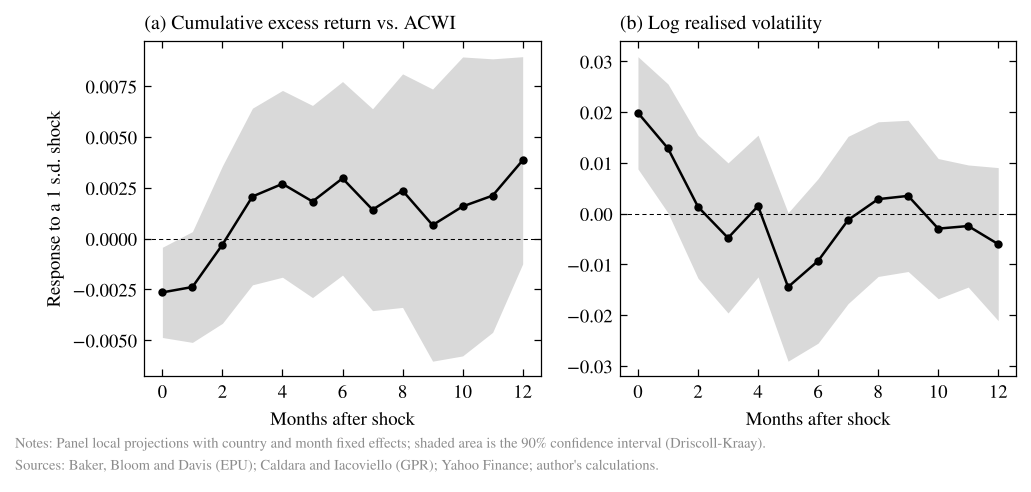
\includegraphics[width=\textwidth]{fig2_local_projections.png}
\caption{Panel local projections: response to a one-standard-deviation political-risk shock, with 90\% confidence bands.}
\label{fig:lp}
\end{figure}

The panel VAR (Figure~\ref{fig:var}) gives a larger volatility response, about 5.7\% on impact. This is expected, since the VAR does not net out month effects and so includes the part of political risk that moves many markets together, such as the 2022 invasion of Ukraine. The response decays below 1\% within four months but stays statistically above zero for most of the year. The VAR's return response is small and insignificant at every horizon.

\begin{figure}[h]
\centering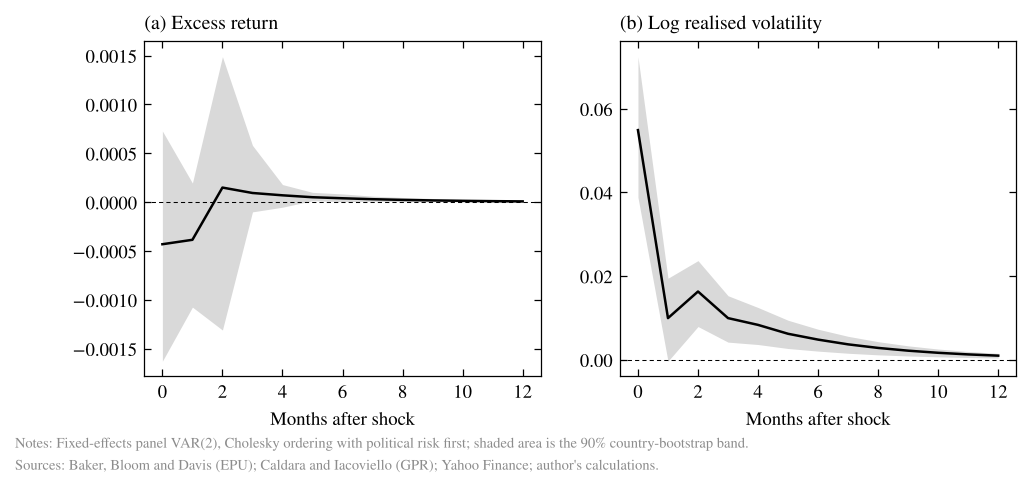
\includegraphics[width=\textwidth]{fig3_panel_var_irf.png}
\caption{Fixed-effects panel VAR(2): impulse responses to a political-risk shock, with 90\% country-bootstrap bands.}
\label{fig:var}
\end{figure}

\subsection{Event type matters more than the event}
Across all 30 events, the mean three-day CAR is $-1.4\%$ (BMP $p = 0.16$). Grouping by event type shows a clear split (Table~\ref{tab:events}). Governance shocks average $-4.8\%$ over three days ($p = 0.02$), led by Brazil's 2017 Temer recording scandal ($-14.0\%$) and South Africa's dismissal of finance minister Nene in 2015 ($-11.7\%$). Policy shocks (the 2011 U.S. downgrade, India's demonetisation and the UK mini-budget) average $-3.1\%$ ($p = 0.05$, three events). Scheduled elections average $+0.8\%$ and are not significant. The Brexit vote ($-7.9\%$) is the main exception, and it was the outcome markets had priced as unlikely.

\begin{table}[h]
\centering\small
\begin{tabular}{lrrrrr}
\toprule
Event type & $n$ & CAR $[-1,+1]$ & BMP $p$ & CAR $[0,+5]$ & BMP $p$ \\
\midrule
Governance    & 8  & $-4.8\%$ & 0.02 & $-3.7\%$ & 0.10 \\
Policy shock  & 3  & $-3.1\%$ & 0.05 & $-3.2\%$ & 0.22 \\
Geopolitical  & 2  & $-1.4\%$ & 0.33 & $-4.2\%$ & 0.58 \\
Unrest        & 3  & $-1.1\%$ & 0.57 & $-0.1\%$ & 0.82 \\
Election      & 14 & $+0.8\%$ & 0.46 & $+0.8\%$ & 0.35 \\
\midrule
All events    & 30 & $-1.4\%$ & 0.16 & $-1.2\%$ & 0.24 \\
\bottomrule
\end{tabular}
\caption{Mean cumulative abnormal returns by event type, market model on ACWI, Boehmer--Musumeci--Poulsen test.}
\label{tab:events}
\end{table}

\begin{figure}[h]
\centering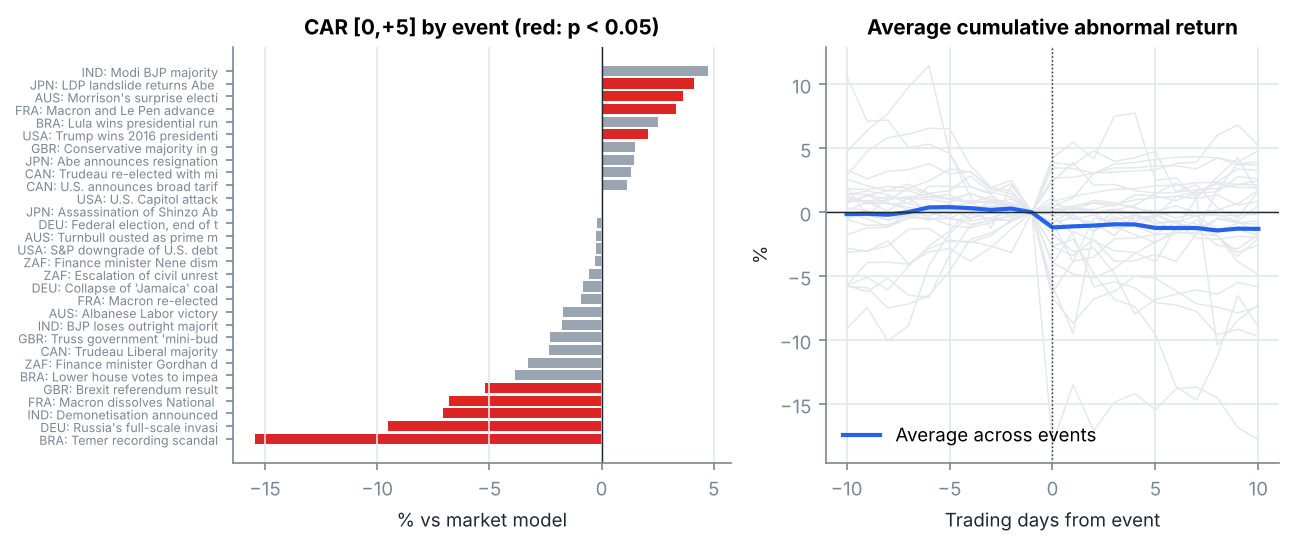
\includegraphics[width=\textwidth]{fig4_event_study.png}
\caption{Event study. Left: CAR over $[0,+5]$ for each event (red: $p < 0.05$). Right: cumulative abnormal returns from $-10$ to $+10$ trading days.}
\end{figure}

\subsection{Portfolio applications}
\textbf{Regimes.} Ranking markets each month by real-time PRI, the top third returned 0.5\% a year more than the bottom third over the next month ($p = 0.83$), with similar realised volatility (21.9\% vs.\ 22.8\%). The \emph{level} of political risk relative to peers carries no information about next month's outcomes; the \emph{surprise} does, through volatility.

\textbf{Tilt backtest.} Starting from an equal-weight country portfolio, I halve the weight of the three markets with the largest three-month rise in real-time PRI and redistribute the rest, using only information available at the start of each month (Table~\ref{tab:bt}). The tilt improves return/volatility slightly, from 0.28 to 0.30, and the maximum drawdown from $-48.2\%$ to $-46.0\%$. With an information ratio of 0.16 and 12.6\% monthly turnover, however, the gain would not survive realistic trading costs.

\begin{table}[h]
\centering\small
\begin{tabular}{lrrrrrr}
\toprule
 & Return & Volatility & Return/vol & Max DD & Tracking error & Info.\ ratio \\
\midrule
Equal weight         & 5.4\% & 19.3\% & 0.28 & $-48.2\%$ & -- & -- \\
Political-risk tilt  & 5.7\% & 19.2\% & 0.30 & $-46.0\%$ & 1.3\% & 0.16 \\
\bottomrule
\end{tabular}
\caption{Backtest, May 2008 -- July 2026, annualised, USD, before costs.}
\label{tab:bt}
\end{table}

\textbf{Stress tests.} Figure~\ref{fig:stress} shows market returns in five political-stress windows. The losses concentrate where the shock originated or where the exposure was largest: the UK ($-13.2\%$) and continental Europe around Brexit; Germany ($-15.6\%$) and France ($-13.7\%$) during the first two weeks of the war in Ukraine, while Canada was flat; Brazil ($-10.2\%$) and South Africa ($-8.1\%$) after the 2016 U.S. election, as the dollar strengthened. An equal-weight portfolio lost between 0.5\% and 6.4\% in each episode. Since returns are in U.S. dollars, much of the emerging-market loss is currency.

\begin{figure}[h]
\centering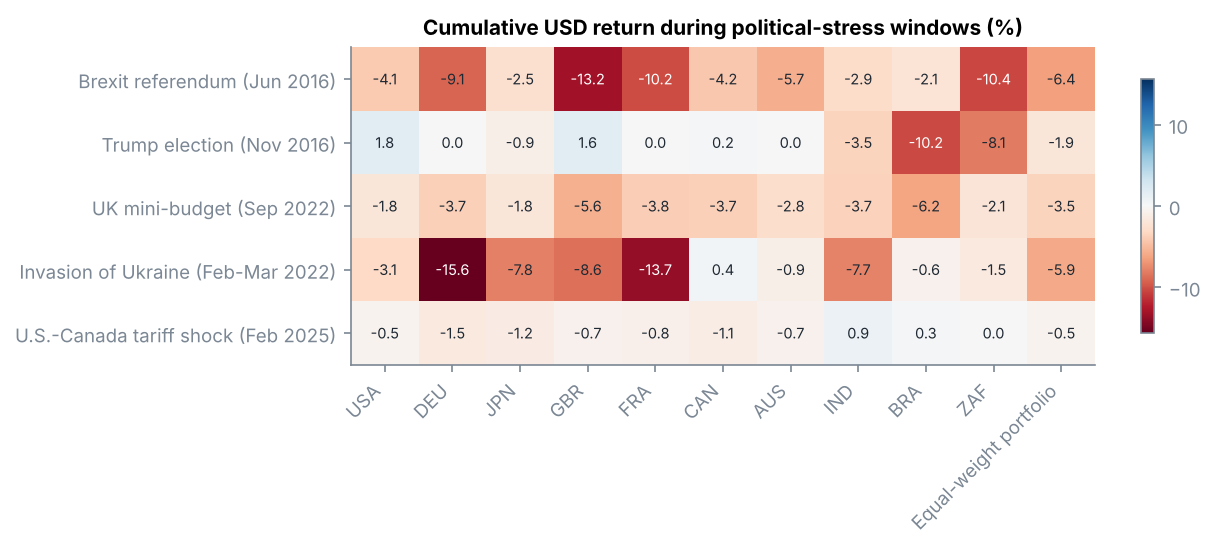
\includegraphics[width=\textwidth]{fig7_stress_tests.png}
\caption{Cumulative USD returns during political-stress windows.}
\label{fig:stress}
\end{figure}

\subsection{Scenarios: what to do if \ldots}
The results above are backward-looking. To turn them into forward-looking guidance, I define four scenarios, each calibrated to a historical episode: tariff escalation (February to April 2025), a European security crisis (the 2022 invasion of Ukraine), a U.S. fiscal standoff (the 2011 debt-ceiling downgrade) and an emerging-market governance shock (Brazil in May 2017, South Africa in December 2015). In each scenario, a country's shock is its largest political-risk surprise in the analogue months, so the scenario reflects how risk actually spread across countries. The panel VAR turns each shock into projected volatility. Holding the last year's correlations fixed, this gives the change in one-month 95\% value at risk (VaR) for an equal-weight portfolio of the ten markets held by a Canadian-dollar investor (Figure~\ref{fig:scn}, Table~\ref{tab:scn}). Correlations usually rise in a crisis, so these figures are a lower bound.

\begin{table}[h]
\centering\small
\begin{tabular}{lrrrl}
\toprule
Scenario & Current VaR & Scenario VaR & Exposure cut & Largest volatility rises \\
\midrule
Tariff escalation          & 7.3\% & 8.2\% & 10.5\% & CAN $+18\%$, JPN $+16\%$ \\
European security crisis   & 7.3\% & 8.1\% & 10.2\% & USA $+18\%$, AUS, GBR $+16\%$ \\
U.S. fiscal standoff       & 7.3\% & 7.8\% & 6.5\%  & ZAF $+10\%$, BRA $+9\%$ \\
EM governance shock        & 7.3\% & 7.3\% & 0.2\%  & not captured by the index \\
\bottomrule
\end{tabular}
\caption{Scenario results: one-month 95\% VaR of an equal-weight portfolio for a Canadian-dollar investor, and the cut in exposure needed to keep VaR at its current level.}
\label{tab:scn}
\end{table}

\begin{figure}[h]
\centering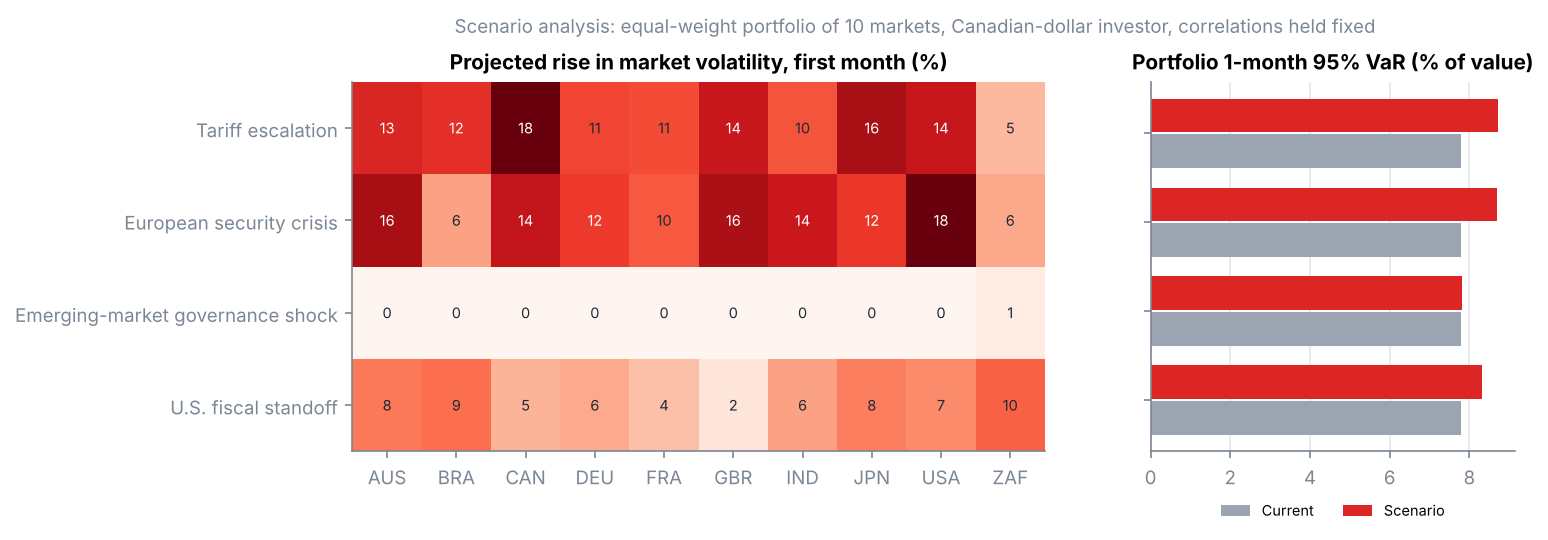
\includegraphics[width=\textwidth]{fig8_scenarios.png}
\caption{Scenarios. (a) Projected rise in each market's volatility in the first month of each scenario; for example, tariff escalation raises Canada's volatility by 18\%, from about 14\% today. (b) The portfolio's one-month 95\% VaR in each scenario, and the cut in exposure that brings it back to today's 7.3\%.}
\label{fig:scn}
\end{figure}

The historical analogues show what the model cannot: how losses split between equity and currency for a Canadian investor (Figure~\ref{fig:fx}). Three findings stand out.
\begin{itemize}
\item \textbf{The U.S. dollar is not a reliable hedge.} In the 2011 standoff, a crisis that started in the U.S., the U.S. dollar still rose about 5\% against the Canadian dollar and cushioned losses. In the 2025 tariff episode it fell, so U.S. stocks lost a Canadian investor 11.9\%: 7.4\% from the market and 4.9\% from the currency.
\item \textbf{Currency can be half the loss.} In the 2022 European crisis, German stocks lost a Canadian investor 7.1\%, about half of it from the euro. In Brazil in 2017, the real accounted for almost half of a 15.0\% loss.
\item \textbf{The index has a blind spot.} The monthly indices barely registered the Brazilian and South African governance shocks (largest shock 0.2 standard deviations), even though markets fell 14\% and 12\% in three days. Domestic governance risk needs monitoring beyond news-based indices. The event study, not the index, is the guide here.
\end{itemize}

\begin{figure}[h]
\centering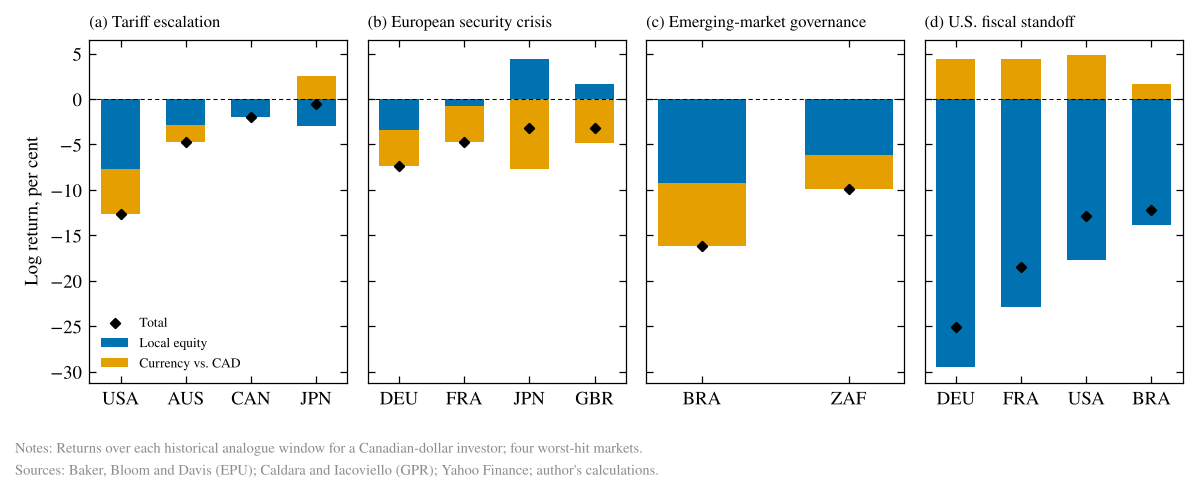
\includegraphics[width=\textwidth]{fig9_scenario_analogues.png}
\caption{Historical analogues: returns of the worst-hit markets for a Canadian-dollar investor, split into local equity and currency against the Canadian dollar.}
\label{fig:fx}
\end{figure}

\subsection{Polls, resignations and three kinds of political risk}
The event study above treats each election as one event. But an election whose result was in the polls for weeks is a different piece of news from one that went against them. Table~\ref{tab:surprise} sorts 50 national elections by how their results compared with the final polls.

\begin{table}[h]
\centering\small
\begin{tabular}{lrrrrr}
\toprule
Poll outcome & $n$ & $|$Equity move$|$ & $\times$ normal day & $|$Currency move$|$ & Significant \\
\midrule
Upset        & 5  & 5.2\% & 5.6 & 3.7\% & 100\% \\
Big miss     & 8  & 2.6\% & 2.4 & 1.3\% & 62\% \\
Toss-up      & 6  & 0.7\% & 1.7 & 0.5\% & 33\% \\
As expected  & 31 & 1.1\% & 1.1 & 1.0\% & 19\% \\
\bottomrule
\end{tabular}
\caption{Average absolute reaction of each country's equities (against ACWI) and currency (against the U.S. dollar) over days 0 to +1, by how the result compared with the final polls. ``Significant'' is the share of equity moves significant at 5\%. Currency moves exclude the United States.}
\label{tab:surprise}
\end{table}

Results that went against the polls moved equities by 3.6 times a normal day's move on average, against 1.1 times for results the polls got right (Welch $p = 0.01$, Mann--Whitney $p < 0.001$). All five upsets moved markets significantly: the Brexit referendum ($-8.7\%$), Trump in 2016, Morrison's win in Australia in 2019, the French legislative run-off in 2024 ($-2.6\%$) and Brazil's 2026 first round ($+10.7\%$). Big misses ranged from India's BJP losing its majority in 2024 ($-3.8\%$) to Japan's 2026 supermajority ($+3.4\%$). Large political changes that the polls had signalled barely moved markets: Japan's ruling coalition losing its majority in 2024 ($+1.2\%$) and South Africa's ANC losing its majority ($+0.3\%$). Currencies also moved more after surprises (4.6 against 1.2 times a normal day for upsets and expected results), but with few currency observations the difference is not significant.

Resignations and ousters of heads of government matter even less (Figure~\ref{fig:surprise}, panel b). Only 3 of 22 moved their market significantly: Suga's decision not to run in 2021 ($+3.8\%$), Starmer's resignation in 2026 ($+2.0\%$) and Lecornu's resignation in 2025 ($-2.4\%$). The UK's five prime-ministerial exits since 2010 moved UK equities by between $-0.8\%$ and $+2.0\%$ against ACWI. By the time a leader goes, the crisis is usually already priced.

\begin{figure}[h]
\centering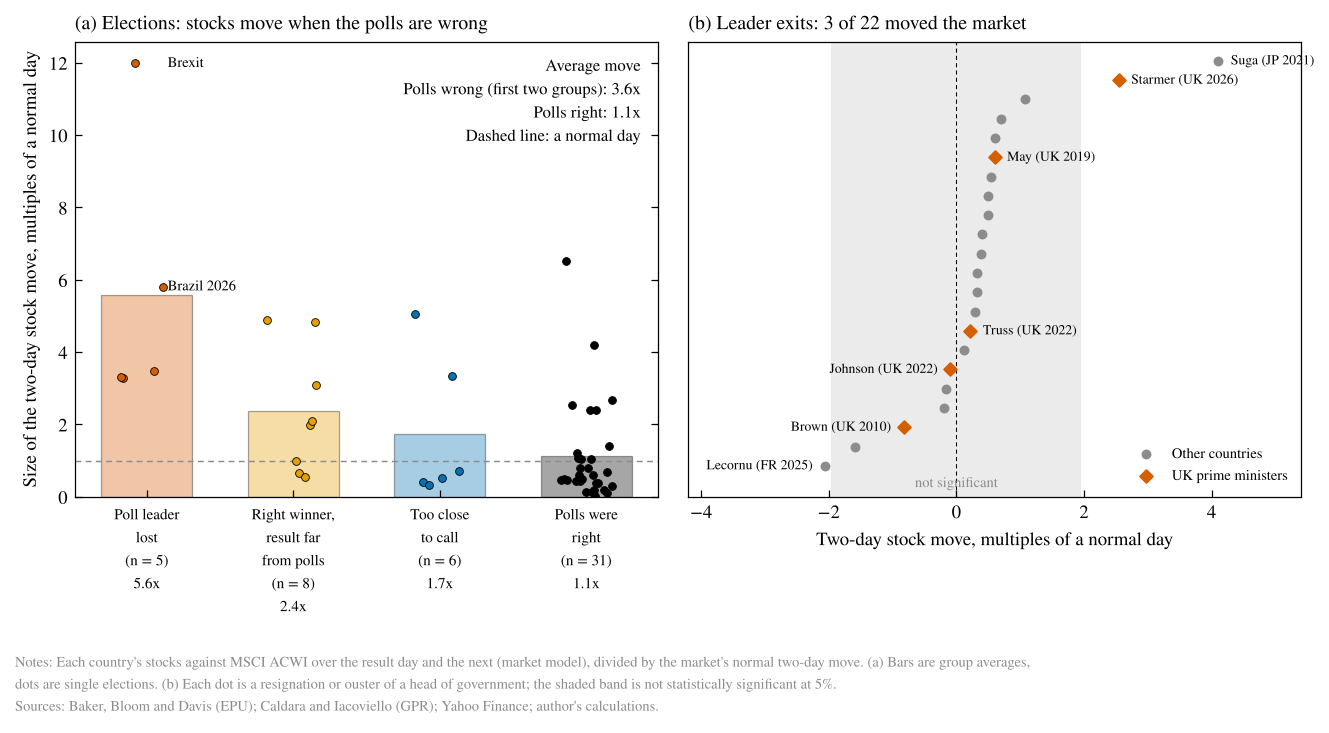
\includegraphics[width=\textwidth]{fig10_election_surprises.png}
\caption{(a) Size of each country's two-day stock move after 50 elections, grouped by how the result compared with the final polls. (b) Two-day stock moves after 22 resignations and ousters of heads of government; only three fall outside the band of normal variation.}
\label{fig:surprise}
\end{figure}

Grouping every dated event by whether its date was known gives a simple taxonomy (Figure~\ref{fig:taxonomy}). \emph{Event risks} with an expected outcome ($n = 41$) average 1.2 times a normal day, and only 20\% are significant. Event risks with a surprise outcome ($n = 14$) average 3.7 times, 79\% are significant, and about 45\% of the typical move reverses within ten days. \emph{Exogenous risks} ($n = 31$) are smaller on impact (1.4 times) but different in kind: they lose 1.0\% on average, the first move tends to keep going, and abnormal-return volatility stays 1.4 times normal for the following ten days, against 1.1 after an expected event.

\begin{figure}[h]
\centering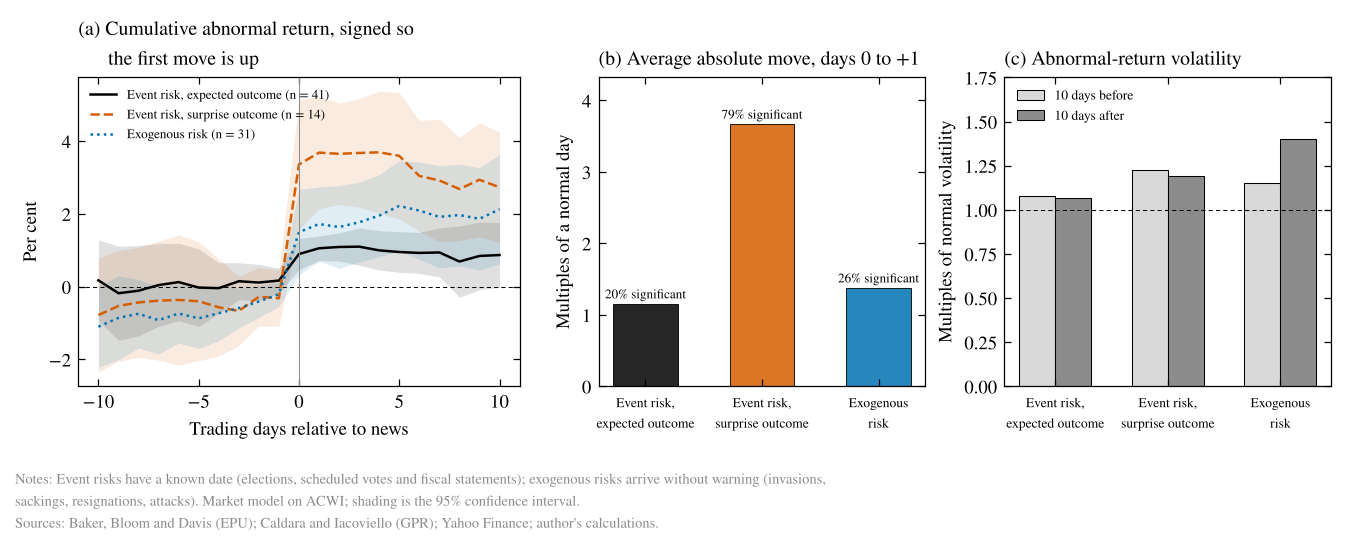
\includegraphics[width=\textwidth]{fig11_risk_taxonomy.png}
\caption{Event risks with expected and surprise outcomes against exogenous risks: average signed path (a), size of the first move (b), and volatility before and after (c).}
\label{fig:taxonomy}
\end{figure}

\emph{Thematic risks} do not show up as one large day at all (Figure~\ref{fig:themes}). French equities lagged ACWI by 26\% from the June 2024 dissolution to October 2026, UK equities by 23\% between the referendum and Brexit, and Brazilian equities by 20\% in the 2014--16 political and fiscal crisis, with the real down a further 23\%. For the nine moves larger than 10\%, no more than 31\% had happened after the first month, and in five the market first moved the other way. Not every theme was a loss: South African equities beat ACWI by 19\% through the ``state capture'' years, once the initial shock was priced and the leadership change came into view.

\begin{figure}[h]
\centering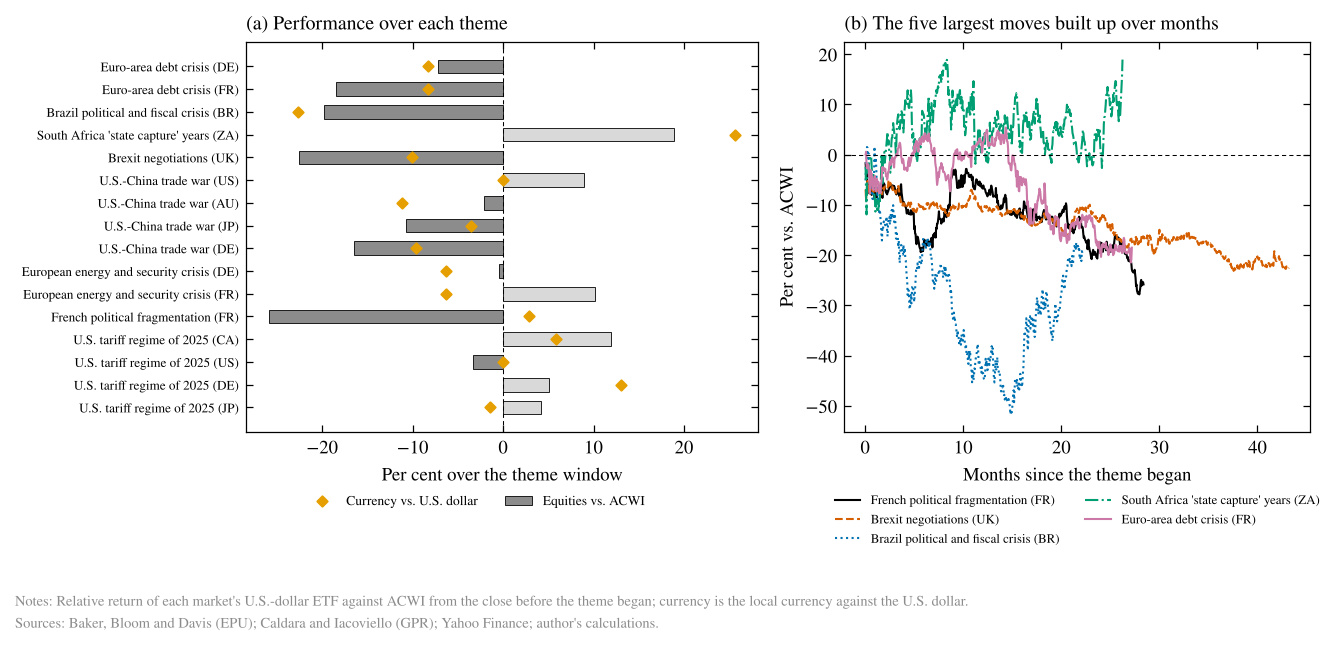
\includegraphics[width=\textwidth]{fig12_thematic_risks.png}
\caption{Thematic risks: performance against ACWI and currency over each theme (a), and how the five largest moves built up (b).}
\label{fig:themes}
\end{figure}

\section{Implications for a total-fund portfolio}
\begin{enumerate}
\item \textbf{Use political risk for sizing, not forecasting.} The robust effect is a short-lived rise in volatility. That is relevant to position sizing, risk limits and the timing of option hedges, but not to return forecasts.
\item \textbf{Watch governance instability, and price the polling error.} Markets price scheduled elections in advance; they move when the polls are wrong. Hedging around an election pays mainly when the polls are close or have a record of missing (referendums, first rounds, seat counts). The large losses otherwise come from unscheduled shocks to who governs or who runs economic policy, which an election calendar would miss.
\item \textbf{Match the response to the kind of risk.} Exogenous shocks belong in the standing risk budget, with liquidity and limits set in advance, because their effect on volatility lasts. Thematic risks build over months and show up in currencies, so they are a strategic allocation and hedging decision rather than a trading one.
\item \textbf{Treat currency as part of the exposure.} For a Canadian-dollar investor, the currency can account for half the loss in a political shock, and the U.S. dollar is a safe haven in some crises but not in others. Hedging decisions should be scenario-specific.
\item \textbf{Pre-agree the risk response.} Tariff escalation or a European security crisis would call for roughly a 10\% cut in exposure to keep value at risk unchanged. Agreeing these responses in advance lets a fund act quickly when a scenario starts to unfold.
\end{enumerate}

\section{Limitations}
Ten markets and 18 years limit statistical power, and some event types have only two or three events. The panel VAR relies on its ordering assumption, which the local projections avoid. EPU and GPR are text-based measures and pick up media attention as well as underlying risk. The event list was chosen by the author and may favour well-known, and therefore larger, episodes. The election surprise classes are judgements from final polls, and there are only five upsets and eight big misses. Theme windows are set by hand and other news moved markets in the same windows. Currency reactions to weekend elections span three trading days because Friday quotes are stale. The backtest excludes transaction costs. The scenarios assume each market responds only to its own political risk and that correlations stay fixed, so they understate risk in a crisis.

\section*{Reproducibility}
All code, data sources and tests are in the \href{https://github.com/divvygupta/political-risk-global-equity-mix}{project repository on GitHub}. Results in this paper are from the October 2026 run; a GitHub Actions workflow refreshes them monthly.

\begin{thebibliography}{9}
\bibitem[Baker et al.(2016)]{bbd2016} Baker, S.~R., Bloom, N., and Davis, S.~J. (2016). Measuring economic policy uncertainty. \emph{Quarterly Journal of Economics}, 131(4), 1593--1636.
\bibitem[Boehmer et al.(1991)]{bmp1991} Boehmer, E., Musumeci, J., and Poulsen, A.~B. (1991). Event-study methodology under conditions of event-induced variance. \emph{Journal of Financial Economics}, 30(2), 253--272.
\bibitem[Caldara and Iacoviello(2022)]{ci2022} Caldara, D., and Iacoviello, M. (2022). Measuring geopolitical risk. \emph{American Economic Review}, 112(4), 1194--1225.
\bibitem[Driscoll and Kraay(1998)]{dk1998} Driscoll, J.~C., and Kraay, A.~C. (1998). Consistent covariance matrix estimation with spatially dependent panel data. \emph{Review of Economics and Statistics}, 80(4), 549--560.
\bibitem[Jord\`a(2005)]{jorda2005} Jord\`a, \`O. (2005). Estimation and inference of impulse responses by local projections. \emph{American Economic Review}, 95(1), 161--182.
\end{thebibliography}
\end{document}
